\documentclass[letterpaper, 12pt]{article}
\usepackage[top=2cm,bottom=1cm,left=0.75in,right=0.75in,headheight=17pt, % as per the warning by fancyhdr
includehead,includefoot,
heightrounded, % to avoid spurious underfull messages
]{geometry}
\addtolength{\topmargin}{-.25in}
\usepackage{fancyhdr}
\pagestyle{fancy}
\usepackage{graphicx}
\usepackage{lastpage}
\usepackage{gensymb}
\usepackage{csquotes}
\usepackage{hyperref}
\usepackage{xcolor}
\usepackage{float}
\usepackage{amsmath}
\usepackage{cancel}


\begin{document}


	\title{The Work-Energy Theorem}
	\author{Jonas Williamson}

\maketitle

\begin{abstract}
	Insert Abstract Here
\end{abstract}
	





\section{Introduction}

After some debate about a question concerning the Work-Energy Theorem, and how it is taught in YISD schools, the need for a study of state and district resources concerning the Work-Energy Theorem became apparent.  

\section{A Survey of Existing State and District Resources}
This section attempts to identify and compare all state and district resources that mention the Work-Energy theorem and trace their development.  

\subsection{Texas Essential Knowledge and Skills}
  The only mention of the Work-Energy Theorem in the Texas Essential Knowledge and Skills for Physics (TEKS) is as follows:
\begin{displayquote}
\textit{(6) Science concepts. The student knows that changes occur within a physical system and applies the laws of conservation of energy and momentum. The student is expected to:}

\textit{(A) investigate and calculate quantities using the work-energy theorem in various situations;} \footnote{\color{blue}\href{http://ritter.tea.state.tx.us/rules/tac/chapter112/ch112c.html}{Texas Education Agency (2017). TEKS, $\S$112.39: Physics}\color{black}} 
\end{displayquote}

It should be noted that the states standards do not define what the Work-Energy Theorem is.  

\subsection{STAAR}\label{STAAR}
Though the State of Texas Assessment of Academic Readiness (STAAR) Physics End-of-Course (EOC) test is no longer required for graduation, there is one released STAAR test that is posted on the Texas Education Agency's website. The reference materials contain the following formula:

\begin{equation}
	W = \Delta KE
\end{equation}
with the words ``Work = change in kinetic energy."\footnote{\color{blue}\href{https://tea.texas.gov/sites/default/files/STAAR-EOC-TestPhysics.pdf}{Texas Education Agency (2013).  STAAR Physics EOC, p. 4}\color{black}}


Also of note is one question on this exam:
\begin{figure}[H]
	\fbox{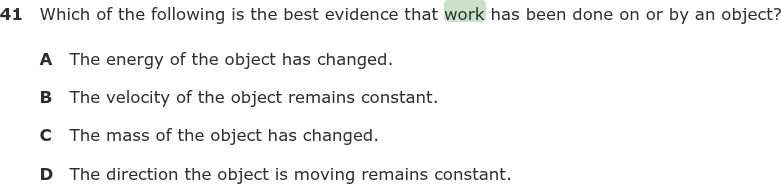
\includegraphics[width=6in]{q41.png}}
	\caption{Question 41 from the 2013 STAAR Physics EOC} 
\end{figure}

The correct answer to this question question\footnote{\color{blue}\href{https://tea.texas.gov/sites/default/files/STAAR-EOC-TestPhysics.pdf}{Texas Education Agency (2013).  STAAR Physics EOC, p. 34}\color{black}} mentions energy, but not kinetic energy specifically.  


\subsection{TEKS Resource System}
The TEKS Resource System was developed by the Texas Curriculum Management Program Cooperative (TCMPC), formed by an agreement by all 20 Education Service Centers in Texas; neither the Texas Education Agency nor the State Board of Education were involved in its development. The TEKS Resource System was originally named C-SCOPE, and changed its name to TEKS Resource System in August of 2013.\footnote{\color{blue}  \href{https://tea.texas.gov/about-tea/leadership/cscope-review}{Texas Education Agency (n.d.). CSCOPE Review} \color{black} }

Both the TEKS Clarification Document\footnote{\color{blue} \href{https://www.teksresourcesystem.net/module/content/search/~/item/694111/viewdetail.ashx}{TEKS Resource System (n.d.) Physics TEKS Clarification Document (Login Required)} \color{black}} and the Unit 5 Instructional Focus Document \footnote{\color{blue}} state the following concerning the Work-Energy Theorem (The text is identical in both documents, so it is only shown here once):

\begin{figure}[H]
	\includegraphics[width=6in]{ifd.png}
\caption{Excerpt from the Unit 6 Instructional Focus Document.}	
\end{figure}

It is clearly seen that these documents define the work energy theorem as: 
\begin{equation}
	W = \Delta {KE}
\end{equation}
	
	In the notes section, the STAAR Physics Reference Materials are mentioned (see STAAR, Section \ref{STAAR} on page \pageref{STAAR}).   It is thus likely that the documents of the TEKS Resource system were developed from the STAAR Reference materials. 
	
	
\subsection{College Board and the AP Tests}

The AP Physics 1 course and exam description Essential Knowledge 5.B.5 lists the following equation:\footnote{\color{blue}\href{https://apcentral.collegeboard.org/pdf/ap-physics-1-course-and-exam-description.pdf?course=ap-physics-1-algebra-based}{College Board, 2020,  AP Physics 1 Course and Exam Description, p. 89}\color{black}}
\begin{equation}
	\Delta E = W = F_{\|} d = Fd\cos{\theta}
\end{equation}

Note that there is no mention of Kinetic energy specifically, only that work is a change in energy.  The same formula is found on the AP Physics 1 Formula Sheet.\footnote{\color{blue}\href{https://apcentral.collegeboard.org/pdf/physics-1-equations-sheet-2020.pdf}{College Board, 2020,  AP Physics 1 Table of Information, p. 2}\color{black}}


\subsection{Textbooks adopted by YISD}
\subsubsection{McGraw-Hill}
The textbook that YISD has adopted for its physics courses is McGraw-Hill's \textit{Physics, Principles \& Problems}.  This book states that ``Work done on a system is equal to the change in the system's energy''  and offers the following formula: 
\begin{equation}
	W = \Delta E
\end{equation}

The text goes on to state, ``There are, however, many other forms of energy.  Work can cause a change in these other forms, as well.''\footnote{McGraw-Hill Education, 2015.  Physics, Principles \& Problems, p. 270.}
\subsubsection{Cutnell \& Johnson}
\textit{Physics, 9e} by Cutnell \& Johnson is the book most recently adopted by YISD for AP Physics 1 and 2 courses.  This book defines the work-energy theorem as follows: 

\begin{displayquote}
	When a net external force does work $w$ on an object, the kinetic energy of the object changes from its initial value of $KE_0$ to a final value of $KE_f$, the difference of the two values being equal to the work:\footnote{Cutnell \& Johnson (2012) Physics, 9ed. John Wiley \& Sons Inc., p. 159}
	\begin{equation}
		W = KE_f - KE_0 = \frac{1}{2}mv_f^2 - \frac{1}{2}mv_0^2
	\end{equation}
\end{displayquote}

The text then goes on to state that ``strictly speaking, the work-energy theorem, as given by [this equation] applies only to a single particle..." and references an article by A.B. Arons in \textit{The Physics Teacher}.\footnote{Arons, A. B. (October 1989) \textit{The Physics Teacher} p. 506, as referenced by Cutnell \& Johnson (2012) Physics, 9ed. John Wiley \& Sons Inc., p. 160}  Alas, I have not yet been able to locate the full text of the article referenced.  

\subsection{Observations Concerning State and District Resources}

It is not surprising that there is disagreement concerning what the work-energy theorem is and how to teach it, considering that there is an inconsistency in the way that it is described in various books and resources.  The question most profoundly becomes, ``Does work cause a change in only Kinetic Energy, or can it affect other types of energy as well?''



\section{Counterexamples}
Let us examine the claim that work only effects kinetic energy (and not total energy).  The following counterexamples must be explained:

\subsection{An Object pushed across a surface with friction.}

A force is applied to an object on a surface where friction is not negligible, such that the object moves at a constant speed.  Clearly, work is done by the applied force but the kinetic energy of the object is constant. Friction dissipates the work being done as thermal energy. 


\subsection{An object lifted at a constant rate}
An object has an initial upward vertical velocity in a gravitational field. A force is applied to the object such that its velocity remains constant.  The kinetic energy of the object remains constant as its gravitational potential energy increases.

\subsection{An spring in isolation, pulled from one side}
Consider a spring floating in empty space, under the influence of no forces.  (It is easier to visualize this with a spring of very low spring constant, such as a slinky, but the spring constant actually doesn't matter much.)  A force is applied to one side of the spring, and it begins to stretch.  While some of the work done by the applied force is transformed into kinetic energy, some of the energy is stored as elastic potential energy as well.  

\subsection{A Piston full of gas, compressed by work}

A force is applied to a piston full of gas, causing the gas to be compressed adiabatically.   The work done increases the internal thermal energy of the gas.  This is supported by the First law of Thermodynamics (sign conventions notwithstanding):

\begin{equation}
	\Delta U = Q + W
\end{equation}

\newpage


\section{Derivations}

\subsection{A Simple Derivation}

The standard derivation of the Work-Energy theorem that incorporates Newton's Second Law is often shown in introductory Physics classes.

We being with the definition of work:
\begin{equation}
	W = \vec{F}\cdot\vec{d}
	\label{eqn:workdef}
\end{equation}

Since newton's Second law states: 
\begin{equation}
	\vec{F} = m \vec{a}
\end{equation}

equation \ref{eqn:workdef} can be expanded to:

\begin{equation}
	W = (m\vec{a})\cdot\vec{d}
	\label{eqn:workexpand}
\end{equation}


One of the basic kinematic equations:
\begin{equation}
	 \overrightarrow{v_f}^2 = \overrightarrow{v_i}^2 + 2 \vec{a} \vec{d}
	\label{eqn:ke4}
\end{equation}

Solving equation \ref{eqn:ke4} for $\vec{d}$ yields:

\begin{equation}
	\vec{d} = \frac{\overrightarrow{v_f}^2 - \overrightarrow{v_i}^2}{2 \vec{a}}
		\label{eqn:ke4mod}
\end{equation}

Substituting this result into equation \ref{eqn:workexpand} and assuming the force acts in the same direction as the displacement gives:

\begin{equation}
	W = m {a} \cdot {d} =  (m \cancel{a}) (\frac{{v_f}^2 - {v_i}^2}{2 \cancel{a}}) = \frac{1}{2}mv_f^2 - \frac{1}{2}mv_i^2 = K_f - K_i 
	\label{eqn:workenergy}
\end{equation}

Thus, 

 \begin{equation}
 	W = \Delta K
 \end{equation}

This naive derivation is problematic for several reasons:
\begin{enumerate}
	\item This definition of work assumes a constant force.
	\item The force in Newton's Second Law is actually a net force ($\Sigma F$), which means if more than one force acts on the object, all external forces must be considered (gravity, friction, etc.)
	\item The use of a kinematic equation in the derivation assumes that the object's acceleration is constant. 
	\item Equation \ref{eqn:ke4mod} has an important restriction that is often overlooked: this equation is not valid for $a = 0 m/s^2$.  Thus the derivation presupposes that the object has a non-zero acceleration.  
	\item This derivation does not allow for the possibility of an extended object that rotates or deforms.  
	
	I suspect that most of our problems come from not understanding the assumptions made in this derivation.  
	
\end{enumerate}

\subsection{A Calculus Based Derivation}
We begin with an integral definition of work, where $r$ is position:
\begin{equation}
	W = \int_{r_i}^{r_f} \vec{F} \cdot \,d\vec{r}
		\label{eqn:workdefcalc}
\end{equation}

We also know that net force is time-derivative of momentum:
\begin{equation}
	\vec{F} = \frac{d\vec{p}}{dt}  
	\label{eqn:forcemomentum}
\end{equation}

Combining these two equations gives: 

\begin{equation}
	W = \int_{r_i}^{r_f} \vec{F} \cdot \,d\vec{r} = \int_{r_i}^{r_f} \frac{d\vec{p}}{dt} \cdot \,d\vec{r} = \int_{pi}^{p_f}  \frac{d\vec{r}}{dt} \cdot d\vec{p} = \int_{p_i}^{p_f} \vec{v} \cdot d\vec{p}  
	\label{eqn:long}
\end{equation}

Using a differential definition of momentum,

\begin{equation}
	d\vec{p} = m \, d\vec{v} 
\end{equation}

We can substitute this definition into equation \ref{eqn:long} to give: 

\begin{equation}
	W = \int_{p_i}^{p_f} \vec{v} \cdot d\vec{p}  = \int_{v_i}^{v_f} \vec{v} \cdot m \, d\vec{v}   
\end{equation}

Assuming the mass of the object is constant, and since $\vec{v}$ and $d\vec{v} $ are in the same direction,  

\begin{equation}
	W = m \int_{v_i}^{v_f} \vec{v} \cdot \, d\vec{v}  = m \frac{v^2}{2} \Big {|}_{v_i}^{v_f} = \frac{mv_f^2}{2} - \frac{mv_i^2}{2} = K_f - K_i = \Delta K
\end{equation}

While this derivation solves the problem of a non-constant force, non-constant acceleration, and is valid for objects of zero acceleration, it still incorporates assumptions 2 and 5 listed above.  


\subsection{A derivation that incorporates Special Relativity}
It is already known that the relativistic definition of momentum is given by the expression

\begin{equation}
	\vec{p} = \frac{m \vec{u}}{\sqrt{1-\frac{u^2}{c^2}}} 
\end{equation}

We also know:
\begin{equation}
	\vec{F} = \frac{d\vec{p}}{dt}
\end{equation}

This derivation begins the same way as the previous one:

\begin{equation}
		W = \int_{r_i}^{r_f} \vec{F} \cdot \,d\vec{r} = \int_{r_i}^{r_f} \frac{d\vec{p}}{dt} \cdot \,d\vec{r} 
\end{equation}

Changing to time domain:

\begin{equation}
	W = \int_{r_i}^{r_f} \frac{d\vec{p}}{dt} \cdot \,d\vec{r}  = \int_{r_i}^{r_f} \frac{d\vec{p}}{dt} \cdot \frac{d\vec{r}}{dt} \,dt   = \int_{p_i}^{p_f} \vec{u} \cdot  d\vec{p}
\end{equation}

\subsection{A derivation by means of the Hamiltonian}


\end{document}
